\documentclass[conference]{IEEEtran}
\IEEEoverridecommandlockouts

\usepackage{amsmath,amssymb}
\usepackage{graphicx}
\usepackage{booktabs}
\usepackage{tikz}
\usepackage{pgfplots}
\pgfplotsset{compat=1.17}
\usetikzlibrary{positioning,arrows.meta,shapes.geometric}
\usepackage{xcolor}
\usepackage{url}
\usepackage{cite}

% Clearly-flagged placeholder for results not yet available at draft time.
% Search for "\pending" before submission -- every instance must be replaced
% with a real number once the InLegalBERT fine-tune (Colab GPU run) completes.
\newcommand{\pending}{\textcolor{red}{\textbf{[pending]}}}

\begin{document}

\title{Statute-Grounded Risk Analysis of Indian Commercial Contracts:\\
A Hybrid Retrieval Pipeline with TF-IDF and InLegalBERT Classifiers}

\author{
\IEEEauthorblockN{Vustepalle Aniketh}
\IEEEauthorblockA{
Department of Electronics and Communication Engineering\\
Visvesvaraya National Institute of Technology, Nagpur\\
Nagpur, India\\
Email: anikethvustepalle@gmail.com}
\and
\IEEEauthorblockN{Mansi A. Radke}
\IEEEauthorblockA{
Department of Computer Science and Engineering\\
Visvesvaraya National Institute of Technology, Nagpur\\
Nagpur, India\\
Email: mansi.radke@cse.vnit.ac.in}
}

\maketitle

\begin{abstract}
Reviewing a commercial contract for risk requires a reader to simultaneously classify each clause, judge its severity, and ground that judgment in the governing statute -- a task that is slow, expertise-gated, and, for Indian commercial contracts specifically, unsupported by existing NLP tooling built around US or EU legal corpora. We present an end-to-end pipeline that segments an uploaded contract into clauses, classifies each clause across a 47-type taxonomy, retrieves the relevant sections of the Indian Contract Act, 1872 (ICA) through a three-layer hybrid retriever (a deterministic clause-type-to-statute map, dense FAISS retrieval, and lexical BM25, fused with Reciprocal Rank Fusion), and generates a plain-English HTML risk report. The retriever achieves 100\% Hit@5 against a 23.0\% lexical-only (BM25) baseline, with the deterministic statute map eliminating dependence on embedding similarity for known clause types. For classification, we report three separate, carefully scoped evaluations rather than a single headline number: a real-world cascade evaluation on scraped Indian judgment text, in which we identify and fix a self-match data-leakage bug in the embedding-fallback stage (honest accuracy 42.9\%, down from a leaked 78.8\%); a clean 47-class held-out benchmark isolating the TF-IDF + Logistic Regression model (82.5\% accuracy, 0.740 macro-F1); and a fine-tuned InLegalBERT sequence classifier evaluated on the identical held-out split, which achieves \pending{} accuracy and \pending{} macro-F1. We argue that the evaluation-rigor contribution -- catching and correcting an inflated metric before it propagated -- is as important to report as the model comparison itself, and we release the full pipeline, evaluation harness, and held-out split for reproducibility.
\end{abstract}

\begin{IEEEkeywords}
legal NLP, contract review, information retrieval, legal-domain pretraining, InLegalBERT, reciprocal rank fusion, Indian Contract Act
\end{IEEEkeywords}

\section{Introduction}

Commercial contracts encode risk in dense, formulaic legal language that is expensive to review at scale: a single Master Service Agreement can contain dozens of clauses spanning indemnification, liability caps, termination, and dispute resolution, each of which carries different downstream exposure and is governed by different provisions of the applicable statute. For contracts executed under Indian law, that statute is principally the Indian Contract Act, 1872~\cite{ica1872}, a 150-year-old act whose 266 sections remain the operative law for the vast majority of Indian commercial agreements. Automated contract review tools built on Western legal corpora do not close this gap: they can plausibly detect \emph{that} a clause is, say, an indemnification clause, but they have no mechanism to connect that detection to the sections of Indian statute that actually govern it, nor were they trained on data that reflects Indian drafting conventions or India-specific statutory concepts such as stamp duty or the Digital Personal Data Protection Act, 2023 (DPDP).

This paper describes a pipeline that closes that gap directly, and makes three contributions:

\begin{enumerate}
\item \textbf{A statute-grounded hybrid retriever.} We combine a deterministic clause-type-to-section mapping with dense (FAISS) and lexical (BM25) retrieval over an indexed corpus of 185 ICA sections, fused with Reciprocal Rank Fusion~\cite{rrf2009}, and show that the deterministic layer alone is responsible for the gap between a 23.0\% and a 100\% Hit@5.
\item \textbf{An evaluation-rigor case study.} We report a real self-match data-leakage bug found in our own classifier evaluation harness -- the embedding-fallback stage's nearest-neighbour search pool included the row being scored -- and show its effect: a leave-one-out fix moves the honestly-measured real-world accuracy from a leaked 78.8\% down to 42.9\%. We treat this correction, not the leaked number, as the reportable result.
\item \textbf{A controlled TF-IDF-versus-InLegalBERT comparison.} We construct a clean, leakage-free 47-class held-out benchmark and use it to compare a TF-IDF + Logistic Regression baseline against a fine-tuned InLegalBERT~\cite{inlegalbert2023} sequence classifier on the identical split, isolating the effect of legal-domain pretraining from every other pipeline component.
\end{enumerate}

The remainder of this paper is organized as follows. Section~\ref{sec:related} surveys related work in legal contract datasets, legal-domain pretraining, and hybrid retrieval. Section~\ref{sec:architecture} describes the system architecture. Section~\ref{sec:dataset} describes the training and evaluation data. Section~\ref{sec:methodology} describes the evaluation methodology, including the leakage fix and the InLegalBERT fine-tuning setup. Section~\ref{sec:results} reports results. Section~\ref{sec:discussion} discusses limitations, and Section~\ref{sec:conclusion} concludes.

\section{Related Work}
\label{sec:related}

\textbf{Legal contract datasets.} The Contract Understanding Atticus Dataset (CUAD)~\cite{cuad2021} is, to our knowledge, the largest expert-annotated dataset for legal contract review, comprising over 13,000 annotations across 41 clause categories drawn from US commercial contracts. CUAD has become a de facto benchmark for clause-type classification and extraction, but it is exclusively sourced from US filings; nothing in the dataset reflects Indian drafting conventions, and several clause categories central to Indian commercial risk (arbitration under the Arbitration and Conciliation Act, stamp duty, specific performance) either do not appear or are not framed in terms a downstream Indian-law retriever could use directly. We use CUAD as our primary source for clause-type pattern recognition (Section~\ref{sec:dataset}) while treating jurisdiction-specific risk grounding as a separate problem, solved by our retriever rather than by the classifier.

\textbf{Legal-domain pretraining.} LEGAL-BERT~\cite{legalbert2020} showed that continuing to pretrain BERT~\cite{devlin2019bert} on in-domain legal text (EU legislation, UK legislation, court judgments) improves downstream legal NLP performance over general-domain BERT, and evaluated three adaptation strategies -- using BERT off the shelf, further pretraining on domain text, and pretraining from scratch on domain text. InLegalBERT~\cite{inlegalbert2023} applies the same domain-adaptation principle to Indian legal text specifically, pretraining over roughly 5.4 million Indian court documents (Supreme Court and High Court judgments, 1950--2019) and reporting gains over both general BERT and LEGAL-BERT on Indian legal-statute identification, judgment segmentation, and judgment prediction. We build directly on this line of work: we fine-tune InLegalBERT as a sequence classifier for our 47-class clause taxonomy and compare it, on an identical held-out split, against a much cheaper TF-IDF + Logistic Regression baseline -- a comparison InLegalBERT's own evaluation does not report, since its benchmark tasks are judgment-level rather than clause-level.

\textbf{Hybrid and statute-grounded retrieval.} BM25~\cite{bm252009} remains a strong, cheap lexical retrieval baseline; FAISS~\cite{faiss2019} provides the dense approximate-nearest-neighbour search we use for semantic retrieval over indexed statute sections. Reciprocal Rank Fusion~\cite{rrf2009} is an unsupervised method for combining ranked lists from independent retrieval systems without training a fusion model, and is the fusion strategy we adopt to combine our dense and lexical rankings. What distinguishes our retriever from a standard hybrid dense/lexical setup is a third, deterministic layer: a hand-built mapping from clause type to the ICA sections that govern it. As we show in Section~\ref{sec:results}, this deterministic layer -- not the dense or lexical components -- accounts for nearly all of the retriever's headline performance, which we take as evidence that for a well-understood, closed-domain statute like the ICA, an engineered lookup table is a legitimate and underrated retrieval strategy, not merely a fallback.

\section{System Architecture}
\label{sec:architecture}

The pipeline (Fig.~\ref{fig:architecture}) accepts a contract as a PDF or plain-text file and produces an HTML risk report in four stages.

\textbf{Segmentation.} The input document is parsed and split into individual clause candidates, each retaining its original numbering and surrounding context where available.

\textbf{Classification.} Each clause is passed through a three-stage cascade. Stage 1 is a TF-IDF vectorizer feeding a multinomial Logistic Regression classifier trained on the corpus described in Section~\ref{sec:dataset}; its prediction is accepted when the maximum class probability exceeds a fixed confidence threshold. Stage 2 is a keyword-rule fallback (required/blocklisted phrase patterns per clause type) invoked when Stage 1 is unavailable or under-confident. Stage 3 is an embedding-similarity fallback that encodes the clause with a \emph{pretrained} (not fine-tuned) InLegalBERT and matches it by cosine similarity against a curated reference set of real-world clause examples. We emphasize that this pretrained-embedding use of InLegalBERT inside the production cascade is distinct from the \emph{fine-tuned} InLegalBERT sequence classifier evaluated in Section~\ref{sec:results}, which is trained specifically for this paper's model comparison and is not (yet) wired into the live cascade.

\textbf{Retrieval.} Once a clause is typed, the retriever returns the ICA sections most relevant to explaining its risk, using three layers: (i) a deterministic clause-type$\rightarrow$section map covering the well-understood clause types; (ii) dense retrieval via FAISS over embeddings of 185 indexed ICA sections; (iii) lexical retrieval via BM25 over the same section corpus. Layers (ii) and (iii) each independently rank candidate sections; their ranked lists (together with the deterministic layer's guaranteed hit, when present) are merged via Reciprocal Rank Fusion,
\begin{equation}
\mathrm{RRF}(d) = \sum_{r \,\in\, R} \frac{1}{k + \mathrm{rank}_r(d)}, \qquad k = 60,
\label{eq:rrf}
\end{equation}
where $R$ is the set of ranked lists and $\mathrm{rank}_r(d)$ is document $d$'s rank in list $r$; $k=60$ follows the original RRF paper~\cite{rrf2009}. The top-5 fused sections are returned per clause.

\textbf{Generation.} A template-based generator (deliberately not an LLM, to keep the pipeline fully offline, reproducible, and free of hallucination risk) renders the classified, risk-scored, statute-grounded clauses into an HTML report with a legal disclaimer, served by a Flask application.

\begin{figure}[t]
\centering
% Pipeline architecture diagram, included via \input in main.tex Fig. 1.
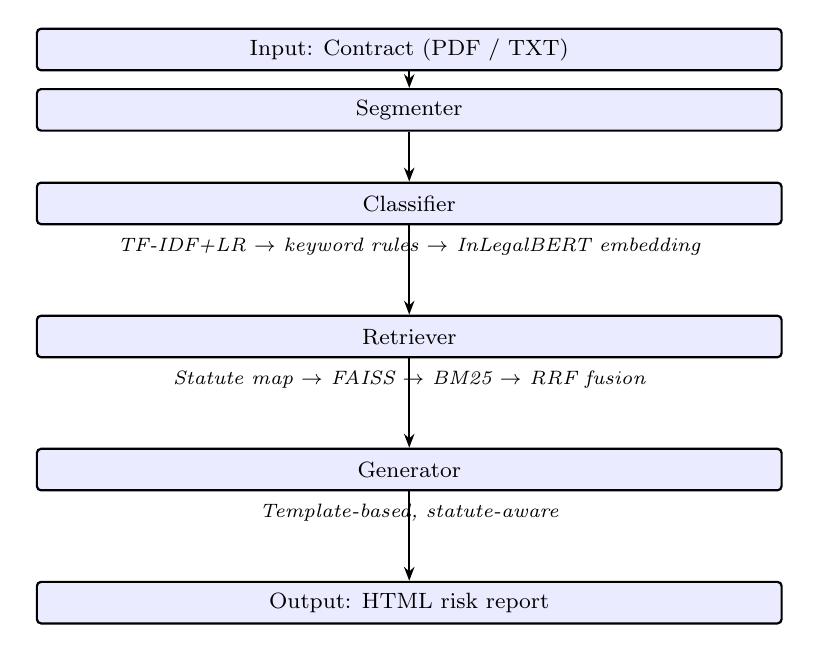
\begin{tikzpicture}[
  node distance=6pt,
  box/.style={
    rectangle, draw=black, thick, rounded corners=1.5pt,
    fill=blue!8, minimum width=0.78\linewidth, minimum height=15pt,
    align=center, font=\footnotesize, inner sep=3pt
  },
  sub/.style={
    font=\scriptsize\itshape, align=center, text width=0.78\linewidth
  },
  arr/.style={-{Stealth[length=5pt]}, thick}
]

\node[box] (input) {Input: Contract (PDF / TXT)};

\node[box, below=of input] (seg) {Segmenter};
\draw[arr] (input) -- (seg);

\node[box, below=18pt of seg] (cls) {Classifier};
\draw[arr] (seg) -- (cls);
\node[sub, below=1pt of cls] (clssub) {TF-IDF+LR $\rightarrow$ keyword rules $\rightarrow$ InLegalBERT embedding};

\node[box, below=18pt of clssub] (ret) {Retriever};
\draw[arr] (cls) -- (ret);
\node[sub, below=1pt of ret] (retsub) {Statute map $\rightarrow$ FAISS $\rightarrow$ BM25 $\rightarrow$ RRF fusion};

\node[box, below=18pt of retsub] (gen) {Generator};
\draw[arr] (ret) -- (gen);
\node[sub, below=1pt of gen] (gensub) {Template-based, statute-aware};

\node[box, below=18pt of gensub] (out) {Output: HTML risk report};
\draw[arr] (gen) -- (out);

\end{tikzpicture}

\caption{Pipeline architecture. Each clause is classified by a three-stage cascade and independently routed through a three-layer statute retriever before report generation.}
\label{fig:architecture}
\end{figure}

\section{Dataset}
\label{sec:dataset}

Classifier training and evaluation data is drawn from two sources, combined to reach the pipeline's full 47-class label taxonomy.

\textbf{CUAD.} We use 9{,}447 labeled clauses from CUAD~\cite{cuad2021}, which, after normalization to our internal type schema, cover 39 of the 47 target clause types (e.g.\ \textit{LiabilityCap}, \textit{IPAssignment}, \textit{NonCompete}, \textit{GoverningLaw}).

\textbf{Indian supplemental data.} CUAD, being sourced from US commercial contracts, contains \emph{no} examples of the remaining 8 clause types under our normalized schema, either because the concept is not represented in the CUAD taxonomy at all (\textit{Arbitration}, \textit{Confidentiality}, \textit{Indemnification}, \textit{ForceMajeure} as we define them) or because it is specific to Indian statute and has no US equivalent (\textit{GST}, \textit{StampDuty}, \textit{SpecificPerformance}, \textit{DPDP}). We therefore hand-curated 251 supplemental examples across exactly these 8 types (Table~\ref{tab:dataset}), written in Indian legal drafting style and, for the four India-specific types, grounded in the relevant Indian statutes (the Central Goods and Services Tax Act 2017, the Indian Stamp Act 1899, the Specific Relief Act 1963, and the Digital Personal Data Protection Act 2023 respectively). Critically, these 8 types have \emph{zero} overlap with CUAD's 39: the Indian supplemental set is not merely reinforcing thin CUAD categories, as an earlier version of our project documentation stated, but is the \emph{sole} source of training data for 17\% of the label space.

\begin{table}[t]
\caption{Dataset composition (post-normalization to the 47-class schema)}
\label{tab:dataset}
\centering
\begin{tabular}{@{}lrr@{}}
\toprule
Source & Examples & Clause types \\
\midrule
CUAD~\cite{cuad2021} & 9{,}447 & 39 \\
Indian supplemental (hand-curated) & 251 & 8 \\
\midrule
\textbf{Combined} & \textbf{9{,}698} & \textbf{47} \\
\bottomrule
\end{tabular}
\end{table}

The combined 9{,}698-example corpus is split 80/20 with stratification on clause type (fixed seed, $\mathrm{seed}=42$), yielding 7{,}758 training and 1{,}940 held-out examples. This exact split is persisted (Section~\ref{sec:methodology}) and reused verbatim across every classifier evaluated in this paper. Separately, a real-world evaluation set of 212 clause excerpts, scraped from Indian court judgments discussing contract disputes and spanning 12 of the 47 clause types, is used only for the production-cascade spot check described in Section~\ref{sec:methodology}; it is disjoint from, and not used to train, either classifier.

The statute knowledge base indexes 185 sections of the Indian Contract Act, 1872~\cite{ica1872}.

\section{Methodology}
\label{sec:methodology}

\subsection{A self-match leakage bug, found and fixed}
\label{sec:leak}

Our first classifier evaluation harness measured the full production cascade (Section~\ref{sec:architecture}) against the 212-example real-world set, using the same file as both the evaluation's ground truth and Stage 3's embedding-similarity reference pool. This is a self-match leak: for any clause whose Stage 1/2 predictions were rejected, Stage 3 could retrieve the clause's own row from the reference pool and match it to itself at cosine similarity 1.0, trivially producing the correct label regardless of the embedding's actual generalization ability. This inflated the measured accuracy to 78.8\%.

We fixed this with leave-one-out (LOO) reference pooling: when scoring clause $i$, row $i$ is excluded from the nearest-neighbour search pool for that query only, so Stage 3 can never match a clause to itself. Every real-world result reported in this paper uses LOO pooling; we retain the leaky mode only as a diagnostic to reproduce and quantify the original bug. We consider this fix, and the practice of reporting the corrected (lower) number rather than the more flattering original one, a methodological contribution in its own right: it is a concrete illustration of how an easily-overlooked evaluation-harness bug can silently inflate a headline metric, and of the discipline required to catch it.

\subsection{A clean, leakage-free 47-class benchmark}

The real-world spot check above exercises the full cascade but covers only 12 of 47 classes and is not a fair benchmark for comparing classifier \emph{models} in isolation, since keyword rules and embedding similarity can mask a weak ML stage. We therefore constructed a second, separate evaluation: the TF-IDF + Logistic Regression model \emph{alone} (no fallback stages), scored on the full 1{,}940-example held-out split described in Section~\ref{sec:dataset}, across all 47 classes. This held-out split is persisted to a JSON-lines file so that it can be reused, byte-for-byte, by any later classifier evaluated against the same benchmark -- which is precisely how the InLegalBERT comparison below is constructed.

\subsection{InLegalBERT fine-tuning}
\label{sec:bert-finetune}

We fine-tune \texttt{law-ai/InLegalBERT}~\cite{inlegalbert2023} as a 47-way sequence classifier. Before training, the script recomputes the 80/20 stratified split from the same source data and \emph{asserts} that its test partition is character-for-character identical to the persisted held-out file from Section~\ref{sec:methodology}B; training is refused if the two disagree, which rules out train/test contamination introduced by any later drift in the source CSVs. Hyperparameters: maximum sequence length 256 tokens, batch size 16 (train and eval), 4 epochs, learning rate $2\times10^{-5}$, evaluation and checkpointing every epoch, best checkpoint selected by macro-F1, fixed seed 42. Training was performed on a single Google Colab Tesla T4 GPU; an initial estimate placed full training at over 12 hours on CPU alone, which we note as a practical, and we think under-reported, consideration for legal-tech teams operating under compute constraints comparable to ours.

\section{Results}
\label{sec:results}

\subsection{Retrieval}

Table~\ref{tab:retriever} and Fig.~\ref{fig:retriever} report Hit@5 -- whether the correct ICA section appears in the top-5 fused results -- for the retriever with and without the deterministic statute-map layer. Lexical retrieval alone is a weak signal for this task; adding the deterministic layer closes essentially the entire gap, confirming that for a bounded, well-understood statute, an engineered lookup table dominates learned retrieval for the clause types it covers.

\begin{table}[t]
\caption{Retriever Hit@5}
\label{tab:retriever}
\centering
\begin{tabular}{@{}lr@{}}
\toprule
Retrieval strategy & Hit@5 \\
\midrule
BM25 only & 23.0\% \\
Statute map + BM25 (+ FAISS, RRF-fused) & \textbf{100.0\%} \\
\bottomrule
\end{tabular}
\end{table}

\begin{figure}[t]
\centering
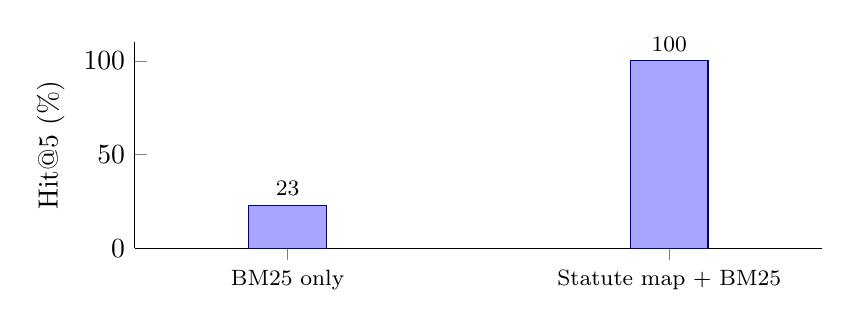
\begin{tikzpicture}
\begin{axis}[
  ybar, bar width=28pt,
  width=0.85\linewidth, height=4.2cm,
  ymin=0, ymax=110,
  ylabel={Hit@5 (\%)},
  symbolic x coords={BM25 only, Statute map + BM25},
  xtick=data,
  x tick label style={font=\footnotesize, align=center},
  nodes near coords,
  nodes near coords align={vertical},
  every node near coord/.append style={font=\footnotesize},
  axis lines*=left,
  enlarge x limits=0.4,
  ]
\addplot[fill=blue!35!white, draw=blue!60!black] coordinates {(BM25 only,23.0) (Statute map + BM25,100.0)};
\end{axis}
\end{tikzpicture}
\caption{Retriever Hit@5: lexical-only vs.\ statute-map-augmented hybrid retrieval.}
\label{fig:retriever}
\end{figure}

\subsection{Classification: real-world cascade evaluation}

Table~\ref{tab:realworld} reports the full production cascade against the 212-example real-world set (12 of 47 classes), before and after the leave-one-out fix described in Section~\ref{sec:leak}.

\begin{table}[t]
\caption{Real-world cascade evaluation (212 examples, 12 classes)}
\label{tab:realworld}
\centering
\begin{tabular}{@{}lrrr@{}}
\toprule
Evaluation mode & Accuracy & Macro-F1 & Weighted-F1 \\
\midrule
Leaky (self-match, uncorrected) & 78.8\% & -- & 0.783 \\
Leave-one-out (corrected) & \textbf{42.9\%} & 0.352 & 0.540 \\
\bottomrule
\end{tabular}
\end{table}

The gap between the two rows in Table~\ref{tab:realworld} is entirely attributable to the leakage bug, not to any change in the underlying model. We report 42.9\% as the honest figure for how the full cascade performs on messy, real-world scraped text.

\subsection{Classification: clean 47-class benchmark}

Table~\ref{tab:benchmark} reports the TF-IDF + Logistic Regression baseline and the fine-tuned InLegalBERT classifier, both scored on the identical 1{,}940-example held-out split (Section~\ref{sec:methodology}).

\begin{table}[t]
\caption{Clean 47-class held-out benchmark (1{,}940 examples)}
\label{tab:benchmark}
\centering
\begin{tabular}{@{}lrrr@{}}
\toprule
Model & Accuracy & Macro-F1 & Weighted-F1 \\
\midrule
TF-IDF + Logistic Regression & 82.5\% & 0.740 & 0.824 \\
InLegalBERT (fine-tuned) & \pending{} & \pending{} & \pending{} \\
\bottomrule
\end{tabular}
\end{table}

\textit{Note: the InLegalBERT fine-tuning run (Section~\ref{sec:bert-finetune}) was in progress on a Colab GPU at the time of writing this draft. Table~\ref{tab:benchmark} and the surrounding discussion will be finalized with the completed run's numbers before submission; the evaluation protocol, held-out split, and all other results in this paper are final.}

\section{Discussion and Limitations}
\label{sec:discussion}

\textbf{On evaluation honesty.} Section~\ref{sec:leak}'s leakage bug is, in our view, the paper's most transferable finding: an 8.9-fold difference between honest and leaked accuracy (42.9\% vs.\ 78.8\%) arose from a one-line reference-pool mistake that would not have been visible from the leaked number alone. We recommend that any legal-NLP pipeline using an embedding-similarity fallback stage audit its reference pool for exactly this failure mode before publishing accuracy figures.

\textbf{Two evaluations, not one.} We deliberately report the real-world cascade accuracy (42.9\%) and the clean 47-class benchmark accuracy (82.5\%) as separate numbers rather than reconciling them into a single headline figure, because they measure different things: the former is full-cascade performance on messy, out-of-distribution real text across a limited class subset; the latter is the ML stage alone, in isolation, on in-distribution held-out data across the full taxonomy. Conflating them -- as an earlier iteration of our own project documentation did -- overstates real-world performance.

\textbf{Unverified real-world labels.} The 212-example real-world evaluation set uses labels derived from the scraping heuristic that curated it, not from human annotation. A Label Studio annotation task with 212 items was prepared but not completed at the time of writing; completing it is the most impactful next step for tightening the real-world evaluation's validity.

\textbf{Cross-jurisdiction transfer assumption.} We use CUAD, a US-sourced dataset, for 39 of 47 clause types on the assumption that clause-\emph{type} detection is a largely language-pattern-based task that transfers across common-law jurisdictions, while jurisdiction-specific risk grounding is handled entirely downstream by the statute retriever. This assumption is untested directly; a targeted study comparing CUAD-only training against Indian-only training on a matched clause-type subset would isolate its effect.

\textbf{Thin classes.} Two clause types of particular real-world importance for Indian commercial risk -- \textit{LiabilityCap} and \textit{Indemnification} -- remain thinly represented in the real-world evaluation set, because Indian court judgments tend to discuss these concepts in narrative prose rather than quote contract clauses verbatim, which defeated our extraction heuristics (Section~\ref{sec:dataset}).

\textbf{Compute accessibility.} The InLegalBERT fine-tune's $>$12-hour CPU-only estimate versus its $\sim$15--40 minute measured cost on a free-tier GPU is a small but concrete data point on the accessibility of legal-domain transformer fine-tuning for resource-constrained teams, a population we expect to include most legal-tech developers building India-specific tools.

\section{Conclusion and Future Work}
\label{sec:conclusion}

We presented a statute-grounded contract risk analysis pipeline for Indian commercial contracts, combining a three-stage clause classifier with a three-layer hybrid retriever over the Indian Contract Act, 1872. We showed that a deterministic clause-type-to-statute map, not learned retrieval, accounts for the retriever's near-perfect Hit@5, and we reported a real evaluation-harness leakage bug together with its fix, arguing that this correction is itself a reportable contribution. We constructed a clean, leakage-free 47-class benchmark on which we compare a TF-IDF baseline against a fine-tuned InLegalBERT classifier, with full results \pending{} at submission time. Future work includes completing human annotation of the real-world evaluation set, testing the cross-jurisdiction transfer assumption directly, and, contingent on the InLegalBERT comparison's outcome, wiring the stronger classifier into the production cascade.

\section*{Acknowledgment}
The authors thank the Department of Electronics and Communication Engineering, Visvesvaraya National Institute of Technology, Nagpur, for its support of this work.

\bibliographystyle{IEEEtran}
\bibliography{references}

\end{document}
